\documentclass[11pt]{article}

\usepackage[a4paper,margin=30mm]{geometry}
\usepackage[T1]{fontenc}
\usepackage{lmodern}
\usepackage{microtype}
\usepackage{amsmath,amssymb,amsthm,mathtools}
\usepackage{booktabs}
\usepackage{graphicx}
\usepackage[numbers,sort&compress]{natbib}
\usepackage{xcolor}
\usepackage{enumitem}
\usepackage{url}
\usepackage[colorlinks=true,linkcolor=blue!55!black,citecolor=blue!55!black,urlcolor=blue!55!black]{hyperref}

\allowdisplaybreaks
\setlist{itemsep=2pt,topsep=4pt}

\newtheorem{theorem}{Theorem}[section]
\newtheorem{proposition}[theorem]{Proposition}
\newtheorem{lemma}[theorem]{Lemma}
\newtheorem{corollary}[theorem]{Corollary}
\theoremstyle{definition}
\newtheorem{definition}[theorem]{Definition}
\newtheorem{remark}[theorem]{Remark}

\newcommand{\Torus}{\mathbb T^3}
\newcommand{\R}{\mathbb R}
\newcommand{\Pp}{\mathbb P}
\newcommand{\curl}{\operatorname{curl}}
\newcommand{\supp}{\operatorname{supp}}
\newcommand{\esssup}{\operatorname*{ess\,sup}}
\newcommand{\ip}[2]{\left\langle #1,#2\right\rangle}
\newcommand{\norm}[1]{\left\lVert #1\right\rVert}
\newcommand{\abs}[1]{\left\lvert #1\right\rvert}
\newcommand{\pos}[1]{\left(#1\right)_{+}}
\newcommand{\dd}{\,\mathrm d}

\title{Projected-Lamb Heat Packing and Sharp Trace Obstructions\\
for Three-Dimensional Navier--Stokes Flow}
\author{Chuikuan Zeng}
\date{26 August 2026}

\begin{document}
\maketitle

\begin{abstract}
For the three-dimensional incompressible Navier--Stokes equations, the
vorticity stretching and transport terms can be compressed into the curl of
the solenoidal Lamb vector
\(L=\Pp(u\times\omega)\).  This paper studies a signed Littlewood--Paley
shell injection built from that representation.  The associated vertical
heat extension has an unconditional bulk estimate: after normalization by
enstrophy, its full heat-height integral belongs to \(L^1\) in physical time
for every periodic Leray--Hopf solution on a finite interval.  The estimate
persists under bounded-overlap spatial localization and yields a conditional
local continuation criterion.

The bulk estimate does not recover the bottom trace.  A fixed smooth radial
tight frame and an explicit global smooth 2D3C Navier--Stokes family give an
exact bottom-to-bulk factor \(2K^2\).  The same family shows that matched
partitions do not hide the loss, while a covariant interior-cylinder
construction rules out every geometry-only factor \(o(r^{-2})\).  A second
construction uses the finite-dimensional implicit-function theorem for the
exact Navier--Stokes flow to prescribe a positive-time full-shell zero with
nonzero nonlinear forcing.  After an amplitude-frequency scaling, its
scale-invariant entry atom is of order \(\lambda^{-4}\), whereas the bare
normalized Leray--Lamb time budget is of order \(\lambda^{-6}\).  Thus no
uniform bare payment of such internal entries is possible.  An outgoing
coarea identity gives an exact scale-matched representation of every
finite-order entry, but its zero-level occupation density is not controlled
here.  None of the results proves global regularity or constructs a
singularity.
\end{abstract}

\medskip
\noindent\textbf{2020 Mathematics Subject Classification.}
35Q30, 35B65, 76D05.

\noindent\textbf{Keywords.}
Navier--Stokes equations; Lamb vector; vorticity stretching; heat extension;
Littlewood--Paley decomposition; trace obstruction; occupation measure.

\section{Introduction}

Let \(u\) be a divergence-free velocity field and
\(\omega=\curl u\) its vorticity.  The obstruction to a direct global
enstrophy estimate in three dimensions is the vortex-stretching work
\(\int S:\omega\otimes\omega\), where
\(S=(\nabla u+\nabla u^{T})/2\).  Classical regularity theory controls this
work by adding geometric coherence, critical-space smallness, or an
integrable strong norm; representative examples include
\citet{Serrin1962}, \citet{ConstantinFefferman1993}, and
\citet{KochTataru2001}.  The aim here is narrower.  I examine one signed
frequency-localized form of the enstrophy injection and determine exactly
which part follows from the Leray energy inequality and which part does not.

The starting identity is classical.  Modulo a Bernoulli gradient, the
Navier--Stokes nonlinearity is the solenoidal Lamb vector
\[
  L=\Pp(u\times\omega)=\partial_tu-\nu\Delta u.
\]
Solenoidal Lamb decompositions have appeared in fluid mechanics and in
mathematical formulations of the curl operator
\cite{Shtilman1992,IyerSreenivasanYeung2022,LernerVigneron2022}.  The
contribution of this paper is not that decomposition by itself.  It is the
specific signed shell quotient below, its energy-level heat packing, and
sharp smooth-solution obstructions to recovering its bottom trace.

\subsection{Main results}

Fix a real-even scalar tight Fourier frame \((T_j)_j\).  For heat height
\(s\ge0\), set
\[
 W_{j,s}=e^{s\Delta}T_j\omega,
 \qquad F_{j,s}=e^{s\Delta}T_jL,
 \qquad D_{j,s}=\norm{\nabla W_{j,s}}_2^2,
\]
and define the complete shell injection
\[
 b_{j,s}=\ip{\curl W_{j,s}}{F_{j,s}}.
\]
The positive shell square function is
\[
 \Theta_s^2
 =\sum_{D_{j,s}>0}\frac{\pos{b_{j,s}}^2}{D_{j,s}}.
\]
The first theorem, proved in Sections~\ref{sec:criterion}--\ref{sec:bulk},
is
\begin{equation}\label{eq:intro-bulk}
 \int_0^\infty\Theta_s^2\dd s
 \le \frac12\norm{L}_{\dot H^{-1}}^2
 \le \frac12\norm{u}_4^4.
\end{equation}
If \(Y(t)=\norm{\omega(t)}_2^2\) and
\[
 \mathcal V(t)=Y(t)^{-1}\int_0^\infty\Theta_s(t)^2\dd s,
\]
with the value zero when \(Y=0\), then every periodic Leray--Hopf solution
satisfies
\begin{equation}\label{eq:intro-time}
 \int_0^T\mathcal V(t)\dd t
 \le \frac{C_S^3}{2\sqrt{2\nu}}\norm{u_0}_2^2\sqrt T.
\end{equation}
This is an unconditional statement at the energy level.  Bounded-overlap
localization gives the corresponding estimate with an overlap constant and
also gives a conditional local continuation criterion.

The bottom value
\[
 A_{\mathrm{sb},+}(t)=\Theta_0(t)^2/Y(t)
\]
is different.  Section~\ref{sec:trace} constructs one fixed dyadically
covariant radial frame and a global smooth 2D3C family for which
\begin{equation}\label{eq:intro-trace}
 A_{\mathrm{sb},+}(0)=2K^2\mathcal V(0).
\end{equation}
The identity survives every nonzero nonnegative smooth cutoff.  At a
parabolic heat height \(h=\theta K^{-2}\), the height average is a fixed
positive fraction of the bottom value.  Matched partitions retain the same
scale law.  A separate whole-space scaling argument places the obstruction
on strictly interior admissible skewed cylinders and rules out a pure
geometry-only bottom-from-bulk factor \(o(r^{-2})\).  The critical
\(Cr^{-2}\) factor is saturated, not rejected.

Section~\ref{sec:entry} addresses a temporal objection to a static trace
example.  Starting from
\[
 U=(0,\cos x_1,\cos x_2),
\]
the exact local Navier--Stokes flow is perturbed in the target shell so that
the entire shell vanishes at a prescribed positive time \(\tau\), while its
nonlinear forcing remains nonzero.  The resulting zero is a genuine simple
internal positive entry.  Choosing a base amplitude
\(a_\lambda=\lambda^{-2}\) and then applying integer Navier--Stokes
dilation gives
\begin{equation}\label{eq:intro-payment}
 \frac{\text{internal entry atom}}
 {\displaystyle\int
   \norm{L_\lambda}_{\dot H^{-1}}^2/Y_\lambda\dd t}
 =\frac{2\nu}{\sinh(2\nu\tau)}\lambda^2+o(\lambda^2).
\end{equation}
The initial kinetic energy and critical \(\dot H^{1/2}\) norm tend to zero,
while the initial enstrophy remains bounded.  Thus the failure is not caused
by a large energy ledger or an initial-time observation face.

The final positive statement is an exact outgoing-coarea representation of
all isolated finite-order entries.  Its density has the correct scale, but it
concentrates at the distinguished zero level.  The Leray inequality does not
provide the required uniform occupation estimate in the present argument.

\subsection{Relation to nearby work}

The heat-extension viewpoint is established in critical Navier--Stokes
theory, most notably in the \(BMO^{-1}\) framework of
\citet{KochTataru2001}.  The present square function is solution-dependent,
signed before squaring, and normalized by enstrophy; it is not the
Koch--Tataru norm.  Rigorous skewed-cylinder geometry is available from
\citet{Yang2020} and has been used for derivative estimates by
\citet{VasseurYang2021}.  Those covering theorems do not by themselves
recover a boundary value in the independent heat-height variable.  Recent
caloric trace estimates recover boundary regularity from stronger interior
derivative norms \cite{ChenLiangTsai2026}, rather than from the zero-order
bulk in \eqref{eq:intro-bulk}.

The closest filtered-vorticity comparison located in the preparation of this
draft is \citet{Yu2026}.  That work controls a positive near-field stretching
part and obtains conditional unweighted closure under additional far-field,
commutator, and localization summability.  The observable and the closure
hypotheses differ from those used here.  Exact commutator identities also do
not imply defect vanishing without an additional compactness or regularity
input; this distinction is familiar from \citet{DuchonRobert2000}.

The paper makes no priority or literature-exhaustion claim.  Its precise
scope is summarized in Section~\ref{sec:discussion}.

\section{Setting and notation}\label{sec:setting}

The periodic part of the paper is set on
\(\Torus=(\R/2\pi\mathbb Z)^3\) with normalized spatial measure.  The
velocity has zero mean and satisfies
\begin{equation}\label{eq:nse}
 \partial_tu+u\cdot\nabla u+\nabla p=\nu\Delta u,
 \qquad \nabla\cdot u=0,
 \qquad \omega=\curl u.
\end{equation}
All Fourier multipliers are set to zero on the zero mode.  The Leray
projection is denoted by \(\Pp\).

A \emph{real-even scalar tight frame} is a countable family of scalar
Fourier multipliers \((T_j)_j\), with symbols \(m_j(k)\), such that
\begin{equation}\label{eq:tight}
 m_j(-k)=m_j(k)\in\R,
 \qquad \sum_j\abs{m_j(k)}^2=1
 \quad (k\ne0).
\end{equation}
For finite frames all sums are literal.  Infinite sums are interpreted by
finite truncation followed by monotone or Fatou convergence whenever the
summands are nonnegative.

The rotational form of \eqref{eq:nse} gives
\begin{equation}\label{eq:lamb}
 u\times\omega=L+\nabla B,
 \qquad
 B=p+\frac12\abs{u}^2,
 \qquad
 L=\Pp(u\times\omega)
   =\partial_tu-\nu\Delta u
   =-\Pp\nabla\cdot(u\otimes u).
\end{equation}
Taking curl yields
\begin{equation}\label{eq:vort-lamb}
 \partial_t\omega-\nu\Delta\omega
 =\curl L=S\omega-u\cdot\nabla\omega.
\end{equation}

For \(s\ge0\), define
\begin{equation}\label{eq:heat-fields}
 A_{j,s}=e^{s\Delta}T_j,
 \quad W_{j,s}=A_{j,s}\omega,
 \quad F_{j,s}=A_{j,s}L,
 \quad D_{j,s}=\norm{\nabla W_{j,s}}_2^2.
\end{equation}
Since \(W_{j,s}\) is divergence free,
\(D_{j,s}=\norm{\curl W_{j,s}}_2^2\).  The heat-extended vorticity equation
is
\begin{equation}\label{eq:heat-vort}
 (\partial_t-\nu\partial_s)W_{j,s}=\curl F_{j,s}.
\end{equation}

\section{A signed shell continuation coefficient}\label{sec:criterion}

At heat height \(s\), define the complete shell work
\begin{equation}\label{eq:shell-work}
 b_{j,s}=\ip{\curl W_{j,s}}{F_{j,s}}.
\end{equation}
This includes stretching and the transport-filter commutator.  Indeed,
\begin{equation}\label{eq:compression}
\begin{aligned}
 b_{j,s}
 &=\ip{W_{j,s}}{A_{j,s}(S\omega-u\cdot\nabla\omega)}\\
 &=\ip{W_{j,s}}
 {A_{j,s}(S\omega)+[u\cdot\nabla,A_{j,s}]\omega}.
\end{aligned}
\end{equation}
The advective pairing with \(W_{j,s}\) vanishes globally.  Pressure is the
gradient complement in \eqref{eq:lamb} and is therefore not a third
independent vorticity work term.

At \(s=0\), write
\begin{equation}\label{eq:Asb}
 \Theta_0^2=\sum_{D_{j,0}>0}\frac{\pos{b_{j,0}}^2}{D_{j,0}},
 \qquad
 A_{\mathrm{sb},+}=\frac{\Theta_0^2}{Y},
 \qquad Y=\norm{\omega}_2^2,
\end{equation}
with value zero when \(Y=0\).

\begin{proposition}[Conditional shell continuation]\label{prop:continuation}
Let \(u\) be a maximal periodic \(H^1\) strong solution on
\([0,T_*)\).  If
\begin{equation}\label{eq:continuation-hyp}
 \int_0^{T_*}A_{\mathrm{sb},+}(t)\dd t<\infty,
\end{equation}
then \(u\) extends beyond \(T_*\).
\end{proposition}

\begin{proof}
Set \(D=\norm{\nabla\omega}_2^2\) and
\(\mathfrak P=\int S:\omega\otimes\omega\).  Tightness gives
\(\sum_jD_{j,0}=D\) and \(\sum_jb_{j,0}=\mathfrak P\).  Positive-part
subadditivity and weighted Cauchy imply
\[
 \mathfrak P_+
 \le \sqrt D\,\Theta_0
 \le \frac\nu2D+\frac1{2\nu}A_{\mathrm{sb},+}Y.
\]
The enstrophy identity therefore yields
\[
 Y'+\nu D\le\nu^{-1}A_{\mathrm{sb},+}Y.
\]
Gronwall and \eqref{eq:continuation-hyp} bound \(Y\) on \([0,T_*)\) and
place \(D\) in \(L^1(0,T_*)\).  The standard strong-solution continuation
theorem then extends the solution; see, for example,
\citet{FujitaKato1964,Kato1984,Temam2001}.
\end{proof}

\begin{remark}
Proposition~\ref{prop:continuation} is a scale-critical conditional
reduction, not an unconditional regularity criterion.  The rest of the paper
tests whether \eqref{eq:continuation-hyp} follows from the energy-controlled
heat extension.
\end{remark}

\section{Unconditional projected-Lamb heat packing}\label{sec:bulk}

For \(s\ge0\), set
\begin{equation}\label{eq:Theta}
 \Theta_s^2
 =\sum_{D_{j,s}>0}\frac{\pos{b_{j,s}}^2}{D_{j,s}}.
\end{equation}

\begin{theorem}[Global heat-bulk estimate]\label{thm:global-bulk}
At every time at which \(u\in H^1(\Torus)\),
\begin{equation}\label{eq:bulk-main}
 \Theta_s^2\le\norm{e^{s\Delta}L}_2^2,
 \qquad
 \int_0^\infty\Theta_s^2\dd s
 \le\frac12\norm{L}_{\dot H^{-1}}^2
 \le\frac12\norm{u}_4^4.
\end{equation}
For a periodic Leray--Hopf solution and every finite \(T\), the normalized
bulk
\begin{equation}\label{eq:Vdef}
 \mathcal V(t)=\frac1{Y(t)}\int_0^\infty\Theta_s(t)^2\dd s
\end{equation}
satisfies \eqref{eq:intro-time}.
\end{theorem}

\begin{proof}
Shellwise Cauchy and \eqref{eq:shell-work} give
\[
 \frac{\pos{b_{j,s}}^2}{D_{j,s}}
 \le\norm{F_{j,s}}_2^2.
\]
Summing and using \eqref{eq:tight} proves the first inequality in
\eqref{eq:bulk-main}.  Since \(L\) has zero mean,
\[
 \int_0^\infty\norm{e^{s\Delta}L}_2^2\dd s
 =\frac12\norm{(-\Delta)^{-1/2}L}_2^2.
\]
The multiplier \((-\Delta)^{-1/2}\Pp\nabla\cdot\) has \(L^2\) operator
norm at most one from matrix fields with the Frobenius norm to vector fields.
Equation~\eqref{eq:lamb} therefore gives
\[
 \norm{L}_{\dot H^{-1}}
 \le\norm{u\otimes u}_2=\norm{u}_4^2.
\]
This proves \eqref{eq:bulk-main}.

The three-dimensional interpolation and Sobolev inequalities give
\[
 \norm{u}_4^4
 \le\norm{u}_2\norm{u}_6^3
 \le C_S^3\norm{u}_2Y^{3/2}.
\]
Hence
\[
 \mathcal V(t)\le\frac{C_S^3}{2}\norm{u(t)}_2Y(t)^{1/2}.
\]
The Leray inequality implies
\[
 \norm{u(t)}_2\le\norm{u_0}_2,
 \qquad
 \nu\int_0^TY(t)\dd t\le\frac12\norm{u_0}_2^2.
\]
Cauchy in time proves \eqref{eq:intro-time}.

For weak solutions, the argument is first applied to finite shell and
heat-height truncations at almost every \(H^1\) time.  Tonelli and Fatou then
give the stated interpretation.  No solution-dependent test function is
inserted into the weak formulation.
\end{proof}

The factorization of the unresolved trace is now explicit.  When the
denominator is positive, define
\begin{equation}\label{eq:Lambda}
 \Lambda_L^2(t)=
 \frac{\Theta_0(t)^2}{\displaystyle\int_0^\infty\Theta_s(t)^2\dd s};
\end{equation}
otherwise set \(\Lambda_L=0\).  Then
\begin{equation}\label{eq:factorization}
 A_{\mathrm{sb},+}=\Lambda_L^2\mathcal V.
\end{equation}
Theorem~\ref{thm:global-bulk} controls \(\mathcal V\), but does not control
\(\Lambda_L^2\).

\section{Bounded-overlap localization}\label{sec:local}

Let \((\chi_{j,Q})_Q\) be a nonnegative smooth partition of unity at the
matched radius \(r_j\simeq K_j^{-1}\), where \(T_j\) is supported in
\(cK_j\le\abs{k}\le CK_j\).  Assume uniform derivative bounds and overlap
at most \(N\).  Define
\begin{equation}\label{eq:local-work}
 B_{j,Q}(t,s)=\ip{F_{j,s}}{\curl(\chi_{j,Q}W_{j,s})},
 \qquad
 d_{j,Q}(t,s)=\norm{\curl(\chi_{j,Q}W_{j,s})}_2^2,
\end{equation}
and set
\begin{equation}\label{eq:local-q}
 q_{j,Q}(t,s)=
 \begin{cases}
 \pos{B_{j,Q}(t,s)}^2/d_{j,Q}(t,s),&d_{j,Q}>0,\\
 0,&d_{j,Q}=0.
 \end{cases}
\end{equation}
The curl in \eqref{eq:local-work} retains the cutoff collar exactly:
\[
 B_{j,Q}
 =\int\chi_{j,Q}F_{j,s}\cdot\curl W_{j,s}
 +\int F_{j,s}\cdot(\nabla\chi_{j,Q}\times W_{j,s}).
\]

\begin{proposition}[Local packing and criterion]\label{prop:local}
Under the preceding assumptions,
\begin{equation}\label{eq:local-pack}
 \sum_{j,Q}q_{j,Q}(t,s)
 \le N\norm{e^{s\Delta}L(t)}_2^2.
\end{equation}
For every \(\alpha>0\),
\begin{equation}\label{eq:alpha-pack}
 \int_0^\infty s^{\alpha-1}\sum_{j,Q}q_{j,Q}(t,s)\dd s
 \le\frac{N\Gamma(\alpha)}{2^\alpha}
 \norm{(-\Delta)^{-\alpha/2}L(t)}_2^2.
\end{equation}
At \(\alpha=1\), the normalized left side belongs to \(L^1(0,T)\) with
the right side of \eqref{eq:intro-time} multiplied by \(N\).

Moreover, if
\begin{equation}\label{eq:Aloc}
 A_{\mathrm{loc},+}(t)
 =\frac1{Y(t)}\sum_{j,Q}q_{j,Q}(t,0)
\end{equation}
is integrable on the maximal strong interval, then the solution continues.
\end{proposition}

\begin{proof}
Cauchy in \eqref{eq:local-work} gives
\[
 q_{j,Q}\le
 \norm{1_{\supp\chi_{j,Q}}F_{j,s}}_2^2.
\]
Bounded overlap and frame tightness prove \eqref{eq:local-pack}.  Spectral
integration gives \eqref{eq:alpha-pack}; the case \(\alpha=1\) then follows
as in Theorem~\ref{thm:global-bulk}.

For the criterion, the matched annular Bernstein and collar bounds imply
\[
 \sum_Qd_{j,Q}\le C_{\chi}\,D_{j,0}.
\]
Since \(\sum_QB_{j,Q}=b_{j,0}\), weighted Cauchy gives
\[
 \frac{\pos{b_{j,0}}^2}{D_{j,0}}
 \le C_{\chi}\sum_Qq_{j,Q}(t,0).
\]
Thus \(A_{\mathrm{sb},+}\le C_{\chi}A_{\mathrm{loc},+}\), and
Proposition~\ref{prop:continuation} applies.
\end{proof}

\begin{remark}
The local criterion is not claimed to be weaker than a standard published
criterion.  Direct Cauchy gives
\(A_{\mathrm{loc},+}\le N\norm{L}_2^2/Y
\le N\norm{u}_\infty^2\), so the Serrin endpoint
\(u\in L_t^2L_x^\infty\) implies it.
\end{remark}

\section{Exact critical trace loss}\label{sec:trace}

The estimates above integrate in the heat-height variable.  This section
shows that the missing boundary trace costs two frequency powers even for
global smooth solutions.

For \(\sigma\in\{-1,1\}\), \(a>0\), and integer \(K\ge1\), define
\begin{equation}\label{eq:2d3c}
 u_{\sigma,a,K}(x)=aK
 \left(0,-2\cos(Kx_1),
 2\sigma\sin(Kx_1+Kx_2)-2\cos(Kx_2)\right).
\end{equation}
This field is real, zero mean, divergence free, and independent of \(x_3\).
Its horizontal velocity is a decaying two-dimensional shear and its third
component solves a linear advection-diffusion equation driven by that shear.
It therefore generates a global smooth three-dimensional periodic solution.

Choose one fixed smooth dyadically covariant radial tight frame that first
places the radii \(K\) and \(\sqrt2K\) in one parent and then splits them
exactly into low and high children.  Such a frame is obtained from a smooth
square partition in \(\log_2\abs{\xi}\) with a flat top, followed by a fixed
sine-cosine refinement.  The frame is fixed before \(K\) is chosen.

For \(\sigma=-1\), the only positive child is the low-radius block.  Direct
Fourier calculation gives
\begin{equation}\label{eq:low-block}
 b_{\mathrm{lo}}(s)=2a^3K^6e^{-2K^2s},
 \quad
 D_{\mathrm{lo}}(s)=4a^2K^6e^{-2K^2s},
 \quad
 q_{\mathrm{lo}}(s)=a^4K^6e^{-2K^2s}.
\end{equation}

\begin{theorem}[Sharp global and localized trace cost]\label{thm:trace}
For the family \eqref{eq:2d3c} and the fixed frame above,
\begin{equation}\label{eq:trace-global}
 q_{\mathrm{lo}}(0)=2K^2\int_0^\infty q_{\mathrm{lo}}(s)\dd s,
\end{equation}
and, with \(Y=8a^2K^4\),
\begin{equation}\label{eq:trace-normalized}
 A_{\mathrm{sb},+}(0)=\frac{a^2K^2}{8},
 \qquad
 \mathcal V(0)=\frac{a^2}{16},
 \qquad
 A_{\mathrm{sb},+}(0)=2K^2\mathcal V(0).
\end{equation}

Let \(\phi\ge0\) be any nonzero smooth cutoff fixed before the data, and
let \(q_\phi\) be defined by the complete localized work in
\eqref{eq:local-work}.  Then for every \(h>0\),
\begin{equation}\label{eq:trace-local}
 q_\phi(0)=\frac{2K^2}{1-e^{-2K^2h}}
 \int_0^h q_\phi(s)\dd s.
\end{equation}
In particular, at \(h=\theta K^{-2}\), the heat-height average is a fixed
positive fraction of the bottom value.
\end{theorem}

\begin{proof}
Equation~\eqref{eq:trace-global} follows by integrating the last formula in
\eqref{eq:low-block}; division by \(Y\) gives
\eqref{eq:trace-normalized}.

For the local statement, the low block is
\[
 W_s=2aK^2e^{-K^2s}(\sin(Kx_2),0,\sin(Kx_1)),
 \quad
 F_s=-2a^2K^3e^{-K^2s}(0,0,\cos(Kx_2)).
\]
The complete localized work, including the cutoff collar, satisfies
\[
 B_\phi(s)=\ip{F_s}{\curl(\phi W_s)}
 =4a^3K^6e^{-2K^2s}
   \int\phi(x)\sin^2(Kx_2)\dd x>0.
\]
Both \(F_s\) and \(W_s\) lie on \(\abs{k}=K\), so
\(q_\phi(s)=e^{-2K^2s}q_\phi(0)\).  Integration over \([0,h]\) proves
\eqref{eq:trace-local}.
\end{proof}

At the matched height,
\begin{equation}\label{eq:trace-fraction}
 \frac{h^{-1}\int_0^h q_\phi(s)\dd s}{q_\phi(0)}
 =\frac{1-e^{-2\theta}}{2\theta}.
\end{equation}
The factor is positive and independent of \(K\).

Matched partitions do not remove the scale.  If
\((\phi_Q)_Q\) is a standard nonnegative partition at radius
\(r=\rho/K\) with overlap \(N\) and uniform square-derivative bounds, then
\begin{equation}\label{eq:partition-two-sided}
 \frac{a^4K^6e^{-2K^2s}}
 {2(C_0+C_1/\rho^2)}
 \le\sum_Qq_Q(s)
 \le2Na^4K^6e^{-2K^2s}.
\end{equation}
Choosing \(a=K^{-1}\) keeps \(\norm{u}_2^2=6\).  The normalized aggregate
bottom remains between positive constants, while its heat bulk is
\(O(K^{-2})\).

\begin{figure}[t]
 \centering
 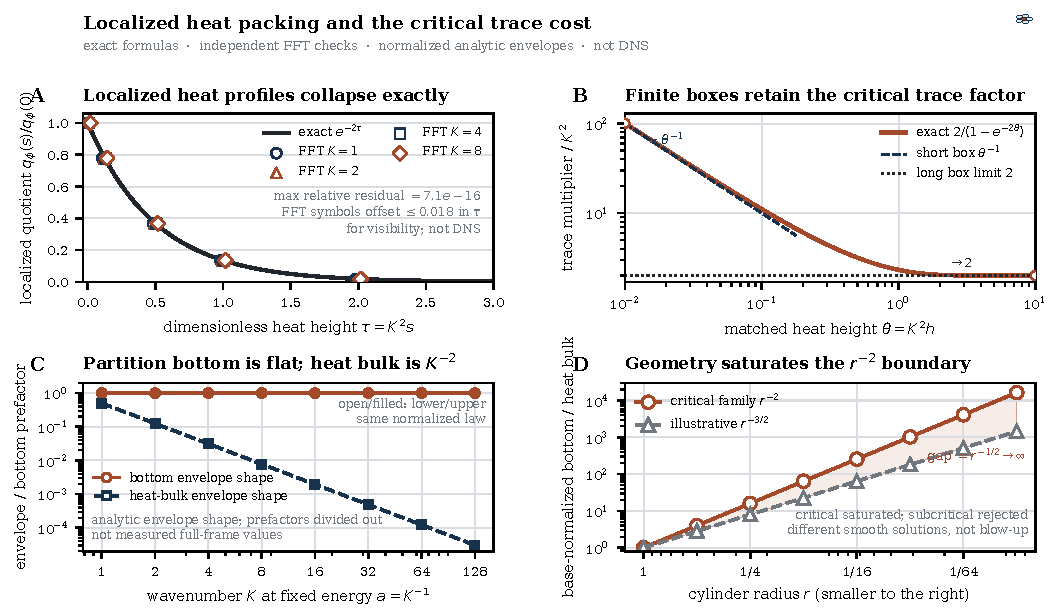
\includegraphics[width=\textwidth,trim=0 15pt 0 28pt,clip]
 {figures/local-trace.pdf}
 \caption{Localized heat packing and the critical trace cost.  The exact
 profile is \(q_\phi(s)/q_\phi(0)=e^{-2K^2s}\).  The finite spectral points
 independently reconstruct the trigonometric identity and are not DNS.
 Matched partitions preserve the bottom scale while the corresponding bulk
 decays by \(K^{-2}\) at fixed kinetic energy.  The last panel shows the
 covariant \(r^{-2}\) interior-cylinder scaling.}
 \label{fig:local-trace}
\end{figure}

\subsection{Interior cylinders}

The exact family above is evaluated at an initial trace.  The same critical
power occurs on strictly interior cylinders, with a narrower conclusion.

\begin{theorem}[Geometry-only subcritical trace no-go]\label{thm:interior}
There is a scale-covariant family of smooth whole-space Navier--Stokes
solutions and strictly interior admissible skewed cylinders \(Q_r\) for
which
\begin{equation}\label{eq:interior-scaling}
 \frac{A_{Q_r}}{\mathcal V_{Q_r,\theta r^2}}=c_*r^{-2},
 \qquad c_*>0.
\end{equation}
Consequently, an estimate
\[
 A_Q\le c(r)\mathcal V_{Q,\theta r^2}
\]
that is required for all smooth solutions and all cylinders in this
covariant one-block class, with constants depending only on the uniform
geometry and admissibility parameters, cannot have \(c(r)=o(r^{-2})\).
\end{theorem}

\begin{proof}
Choose a compactly supported smooth divergence-free datum that agrees in a
ball with
\[
 u_{\mathrm{aff}}=(x_1,-x_2-x_3,0),
 \qquad \omega_{\mathrm{aff}}=(1,0,0).
\]
In the affine core,
\(\curl L=(\omega\cdot\nabla)u-(u\cdot\nabla)\omega=(1,0,0)\).
For a suitable nonnegative cutoff \(\chi\) in the core,
\(B_\chi^L>0\) and the localized denominator is positive.  Smooth local
existence and continuity preserve this at a small positive center time.
Sufficiently small skewed cylinders are admissible in the sense of
\citet{Yang2020}, because their admissibility quantity is bounded by
\(r^2\sup\norm{\nabla u}_\infty\).

Fix one such base cylinder with radius \(r_0\) and heat height
\(h_0=\theta r_0^2\).  Under the exact scaling
\[
 u_\lambda(t,x)=\lambda u(\lambda^2t,\lambda x),
 \quad r_\lambda=\lambda^{-1}r_0,
 \quad h_\lambda=\lambda^{-2}h_0,
\]
the normalized bottom scales as \(\lambda^2A_Q\), while the normalized heat
bulk is invariant.  This is exactly \eqref{eq:interior-scaling}.
\end{proof}

Theorem~\ref{thm:interior} does not reject a critical \(Cr^{-2}\) trace
inequality, a theorem with additional collar or solution-dependent terms, or
a statement on cylinders that stay a fixed positive physical time away from
the initial face as \(r\to0\).

\section{A genuine positive-time internal entry}\label{sec:entry}

The trace obstructions above leave open whether positive-time dynamics could
prevent the relevant shell observable from entering through zero.  This
section constructs such an entry for the exact smooth Navier--Stokes flow.

Let
\begin{equation}\label{eq:seed}
 U(x)=(0,\cos x_1,\cos x_2),
 \qquad
 \Omega=\curl U=(-\sin x_2,0,-\sin x_1).
\end{equation}
The projected Lamb field is
\begin{equation}\label{eq:Fstar}
 F_*=\Pp(U\times\Omega)=(0,0,\cos x_1\sin x_2).
\end{equation}
It is supported on the four modes \((\pm1,\pm1,0)\), hence on
\(\abs{k}^2=2\), while \(U\) lies on \(\abs{k}^2=1\).  Normalized torus
averages give
\begin{equation}\label{eq:seed-ledger}
 \norm{\Omega}_2^2=1,
 \quad \norm{F_*}_2^2=\frac14,
 \quad \norm{\curl F_*}_2^2=\frac12,
 \quad -\Delta F_*=2F_*.
\end{equation}

Let \(E_*\) be the finite-dimensional real divergence-free velocity space
on the target modes and let \(P_*\) be the corresponding projection.  For
smooth data near zero, standard local theory gives a smooth fixed-time map
\(S_t\) on a common interval, with
\begin{equation}\label{eq:flow-derivative}
 DS_\tau(0)h=e^{\nu\tau\Delta}h.
\end{equation}

\begin{theorem}[Smooth internal positive entry]\label{thm:entry}
For every sufficiently small fixed \(\tau>0\), there is \(a_0>0\) and a
smooth map \(z:(-a_0,a_0)\to E_*\) such that
\begin{equation}\label{eq:z-expansion}
 z(a)=-a^2\tau F_*+O(a^3),
\end{equation}
and, for every \(0<\abs a<a_0\), the solution with initial datum
\(u_0^a=aU+z(a)\) is smooth on \([0,2\tau]\) and has a simple positive
target-shell entry at the strictly internal time \(t=\tau\).  Its leading
entry coefficient is
\begin{equation}\label{eq:A-entry}
 A_+(a)=\frac{a^2e^{-2\nu\tau}}4+O(a^3),
 \qquad A_-(a)=0.
\end{equation}
At least one cell in every nonnegative covering partition also has a simple
positive entry at that time.
\end{theorem}

\begin{proof}
Define
\[
 \Phi(a,z)=P_*S_\tau(aU+z).
\]
At the origin,
\(D_z\Phi(0,0)=e^{-2\nu\tau}I_{E_*}\), an invertible finite matrix.  The
ordinary implicit-function theorem gives a smooth \(z(a)\) with
\(\Phi(a,z(a))=0\).  The quadratic Duhamel term on the target shell is
\[
 e^{\nu(\tau-r)\Delta}P_*
 \Pp\bigl((e^{\nu r\Delta}U)\times
 \curl(e^{\nu r\Delta}U)\bigr)
 =e^{-2\nu\tau}F_*.
\]
Integration in \(r\) gives \eqref{eq:z-expansion}.

At time \(\tau\), the target-shell velocity and vorticity vanish, whereas
the projected Lamb forcing satisfies
\[
 P_*L(u^a(\tau))
 =a^2e^{-2\nu\tau}F_*+O(a^3)\ne0.
\]
Let \(W_*=T_*\omega\) and \(C_*=\curl W_*\).  From the filtered vorticity
equation and \(W_*(\tau)=0\),
\[
 C_{*,t}(\tau)=-\Delta P_*L(u^a(\tau)).
\]
The target forcing is divergence free, annular, and nonzero.  Therefore
\[
 \ip{P_*L(u^a(\tau))}{C_{*,t}(\tau)}
 =\norm{\nabla P_*L(u^a(\tau))}_2^2>0.
\]
The zero is simple and enters from the positive side.  Equations
\eqref{eq:seed-ledger} and the leading low-shell enstrophy give
\eqref{eq:A-entry}.

For a nonnegative partition \((\chi_Q)_Q\), the full-shell root gives
\[
 \ip{P_*L}{C_{Q,t}}
 =\int\chi_Q\abs{\curl P_*L}^2\dd x.
\]
The sum over \(Q\) is positive, so at least one cell has a positive simple
entry.
\end{proof}

\begin{lemma}[Global positive entries are simple]\label{lem:simple}
Every finite-order positive entry of a global nonzero annular shell is
simple.
\end{lemma}

\begin{proof}
At a global-shell zero, \(C_j=\curl W_j=0\).  Since \(W_j\) is divergence
free, annular, and zero mean, this implies \(W_j=0\).  Hence
\(C_{j,t}=-\Delta F_j\).  If the zero had order greater than one, then
\(F_j=0\), contradicting positivity of the entry pairing.  Finally,
\(\ip{F_j}{C_{j,t}}=\norm{\nabla F_j}_2^2>0\).
\end{proof}

\section{No uniform bare payment}\label{sec:no-payment}

For a finite-order entry at \(t_\beta\), write
\[
 C_\beta(t_\beta+s)=c_\beta s^{m_\beta}+O_{L^2}(\abs{s}^{m_\beta+1}),
 \qquad c_\beta\ne0,
\]
and define
\begin{equation}\label{eq:entry-atom}
 A_{\beta,+}
 =\frac{\ip{F_{j(\beta)}(t_\beta)}
 {c_\beta/\norm{c_\beta}_2}_+^2}{Y(t_\beta)},
 \qquad
 a_\beta=\kappa_{j(\beta)}^{-2}A_{\beta,+}.
\end{equation}
Here \(\kappa_j\) is the nominal shell frequency.  The atom \(a_\beta\) is
scale invariant.

For the family in Theorem~\ref{thm:entry},
\begin{equation}\label{eq:bare-base}
 R(a):=\int_0^{2\tau}
 \frac{\norm{L^a(t)}_{\dot H^{-1}}^2}{Y^a(t)}\dd t
 =\frac{a^2(1-e^{-4\nu\tau})}{16\nu}+O(a^3).
\end{equation}
Choose \(a_\lambda=\lambda^{-2}\) and apply the integer periodic scaling
\begin{equation}\label{eq:double-scaling}
 u_\lambda(x,t)=\lambda
 u^{a_\lambda}(\lambda x,\lambda^2t).
\end{equation}

\begin{theorem}[Internal scaling no-go]\label{thm:no-payment}
Along \eqref{eq:double-scaling}, the constructed internal entry and the bare
budget satisfy
\begin{align}
 a_{\beta,\lambda}
 &=\frac{e^{-2\nu\tau}}{4\lambda^4}+O(\lambda^{-6}),
 \label{eq:atom-scale}\\
 R_\lambda
 &=\frac{1-e^{-4\nu\tau}}{16\nu\lambda^6}
   +O(\lambda^{-8}),
 \label{eq:budget-scale}
\end{align}
and therefore
\begin{equation}\label{eq:ratio-scale}
 \frac{a_{\beta,\lambda}}{R_\lambda}
 =\frac{2\nu}{\sinh(2\nu\tau)}\lambda^2+o(\lambda^2).
\end{equation}
There is no constant \(C\), uniform along this family, for which the sum of
internal entry atoms is bounded by \(C R_\lambda\).

Moreover,
\begin{equation}\label{eq:small-data-ledger}
 \norm{u_\lambda(0)}_2^2=O(\lambda^{-2}),
 \qquad
 \norm{u_\lambda(0)}_{\dot H^{1/2}}^2=O(\lambda^{-1}),
 \qquad
 \norm{\omega_\lambda(0)}_2^2=1+o(1).
\end{equation}
\end{theorem}

\begin{proof}
The base entry is given by \eqref{eq:A-entry}.  The covariant dilation moves
it to time \(\tau/\lambda^2\) and preserves the scale-zero atom; the
amplitude choice contributes \(a_\lambda^2=\lambda^{-4}\), proving
\eqref{eq:atom-scale}.  The base budget \eqref{eq:bare-base} acquires the
additional time-scaling factor \(\lambda^{-2}\), which gives
\eqref{eq:budget-scale}.  Their quotient is \eqref{eq:ratio-scale}.

On the normalized torus, the dilation multiplies squared \(L^2\),
\(\dot H^{1/2}\), and \(\dot H^1\) norms by \(\lambda^2\),
\(\lambda^3\), and \(\lambda^4\), respectively.  Combining these factors
with \(a_\lambda^2=\lambda^{-4}\) proves
\eqref{eq:small-data-ledger}.
\end{proof}

\begin{figure}[t]
 \centering
 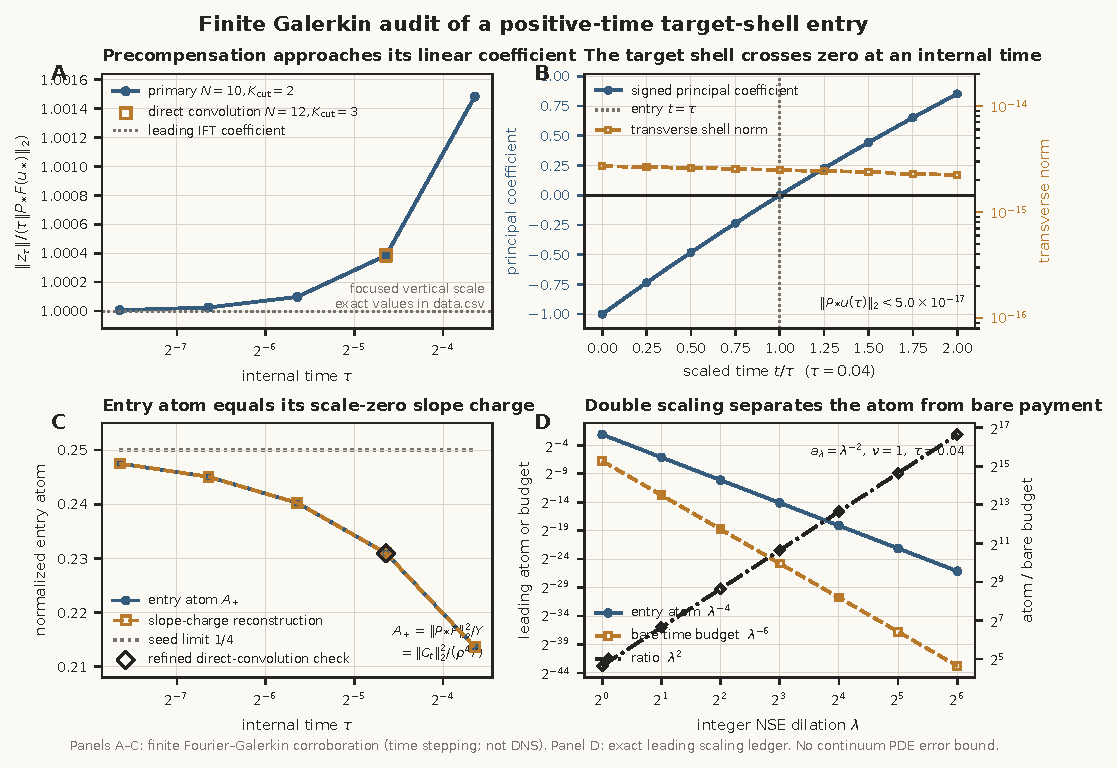
\includegraphics[width=\textwidth,trim=0 16pt 0 22pt,clip]
 {figures/internal-entry.pdf}
 \caption{Finite Fourier--Galerkin corroboration of the internal-entry
 geometry.  Shooting a finite-dimensional target-shell correction makes the
 target shell vanish at \(t=\tau\); the analytic continuum result is
 Theorem~\ref{thm:entry}, not the time stepper.  The last panel displays the
 exact leading powers in Theorem~\ref{thm:no-payment}.}
 \label{fig:internal-entry}
\end{figure}

Theorem~\ref{thm:no-payment} excludes only the bare right side in
\eqref{eq:bare-base} with a constant uniform along the covariant family.  It
does not exclude a fixed-frequency theorem, a constant depending on high
Sobolev norms, or an estimate with an added atomic, variation, strong-Lamb,
or material-derivative charge.

\section{Outgoing occupation at the zero level}\label{sec:occupation}

The bare budget has the wrong scale for an atomic entry.  A zero-level
occupation density has the correct scale and represents the atom exactly.

Let \(I\) be a compact classical interval whose endpoints are not zeros.
For a finite family \(\Lambda\), assume that every zero of every
\(C_\alpha\), \(\alpha\in\Lambda\), is isolated and of finite order.  Put
\begin{equation}\label{eq:occupation-defs}
 r_\alpha(t)=\norm{C_\alpha(t)}_2,
 \qquad
 \xi_\alpha(t)=\frac{C_\alpha(t)}{r_\alpha(t)}\quad(r_\alpha>0),
\end{equation}
and
\begin{equation}\label{eq:qalpha}
 q_\alpha(t)
 =\frac{\ip{F_{j(\alpha)}(t)}{\xi_\alpha(t)}_+^2}{Y(t)}.
\end{equation}
Choose \(\rho\in C_c^\infty((0,1))\), \(\rho\ge0\),
\(\int_0^1\rho=1\), and set \(\rho_\delta(s)=\delta^{-1}\rho(s/\delta)\).

\begin{theorem}[Outgoing-coarea identity]\label{thm:coarea}
Under the preceding assumptions,
\begin{equation}\label{eq:coarea}
\begin{aligned}
 &\sum_{\alpha\in\Lambda}
 \sum_{\substack{t_*\in I\\C_\alpha(t_*)=0}}
 \kappa_{j(\alpha)}^{-2}A_{\alpha,+}(t_*)\\
 &\quad=\lim_{\delta\downarrow0}
 \sum_{\alpha\in\Lambda}\kappa_{j(\alpha)}^{-2}
 \int_Iq_\alpha(t)\rho_\delta(r_\alpha(t))
 \pos{r_{\alpha,t}(t)}\dd t.
\end{aligned}
\end{equation}
The identity includes both odd crossings and even touches.
\end{theorem}

\begin{proof}
Near a zero of order \(m\),
\[
 C(t_*+s)=cs^m+O_{L^2}(\abs{s}^{m+1}),
 \quad
 r(t_*+s)=\norm{c}_2s^m(1+O(s)),
 \quad
 \xi(t_*+s)\longrightarrow c/\norm{c}_2
\]
from the right.  The factor \(\pos{r_t}\) removes the incoming left side.
On the right, the substitution \(y=r(t)\) gives
\[
 \int q(t)\rho_\delta(r(t))\pos{r_t(t)}\dd t
 \longrightarrow q(t_*+)=A_+(t_*).
\]
The argument is unchanged for an even-order touch.  Summing finitely many
disjoint zero neighborhoods proves \eqref{eq:coarea}.
\end{proof}

If \(C_t-\nu\Delta C=G\), then wherever \(r>0\),
\begin{equation}\label{eq:radial}
 r_t=\ip{\xi}{G}-\nu\frac{\norm{\nabla C}_2^2}{r}.
\end{equation}
The density in \eqref{eq:coarea} has scale exponent two before time
integration and therefore total scale zero.  This repairs the dimensional
mismatch of the bare budget only at the level of representation.  The bound
\(\pos{r_t}\le\norm{G}_2\) still leaves
\(\rho_\delta(r)\sim\delta^{-1}\), and no uniform zero-level occupation
estimate follows from an ordinary \(L_t^pG\) bound.

For comparison, a fixed smooth divergence-free packet
\(\psi\) has an amplitude-weighted excursion bound that is paid by the
Leray ledger.  If \(b_\psi(t)=\ip{u(t)}{\psi}\), then on
\(I=[s,t]\),
\begin{equation}\label{eq:excursion}
 V_I^+(b_\psi)
 \le\nu\norm{\nabla\psi}_2(\abs I D_I)^{1/2}
 +\norm{\nabla\psi}_\infty E_I\abs I,
\end{equation}
where
\(E_I=\esssup_I\norm{u}_2^2\) and
\(D_I=\int_I\norm{\nabla u}_2^2\).  This controls entries that reach a
fixed amplitude, not arbitrarily shallow zero entries.

\section{Discussion and exact claim boundary}\label{sec:discussion}

The results isolate a precise separation.

\begin{enumerate}
\item The projected-Lamb shell injection has a complete signed identity and
      a scale-critical conditional continuation coefficient.
\item Leray energy unconditionally controls the normalized vertical heat
      bulk, globally and under bounded-overlap localization.
\item The bottom trace is not a free consequence of that bulk.  Exact global
      smooth solutions saturate the full \(K^2\) trace cost, and covariant
      interior cylinders saturate \(r^{-2}\).
\item Positive-time internal shell entries genuinely occur in smooth
      Navier--Stokes dynamics.  The bare normalized \(\dot H^{-1}\)-Lamb
      time integral cannot uniformly pay their scale-invariant atoms.
\item Outgoing occupation gives an exact scale-matched representation, but
      its summed zero-level mass is an open estimate.
\end{enumerate}

The paper does not prove that \(A_{\mathrm{sb},+}\in L^1_t\) for every
Leray--Hopf solution, does not prove an occupation or recurrence bound, and
does not extend the finite-order entry ledger through an unknown singular
time.  It neither proves global regularity nor constructs finite-time
breakdown.  The remaining question is not another algebraic decomposition:
it is whether the exact Navier--Stokes coupling supplies a scale-zero
occupation, jet, or amplitude-thresholded charge that can be summed from an
a priori budget.

\section*{Reproducibility statement}

The exact Fourier identities, independent reconstructions, figure data,
commands, environments, and checksums are archived in the public repository
\begin{center}
\url{https://github.com/Kasifa/Kasifa.github.io}.
\end{center}
The corresponding certificate directories are linked from the repository's
research index.  Their scripts check finite Fourier
algebra, quadrature identities, and scaling tables.  They do not replace the
continuum proofs based on the local solution map, the implicit-function
theorem, or the Leray inequality.  The time-stepping experiment shown in
Figure~\ref{fig:internal-entry} is a finite Fourier--Galerkin corroboration,
not DNS and not a continuum error certificate.

\appendix
\section{Finite Fourier ledger for the six-mode trace family}

For completeness, the vorticity of \eqref{eq:2d3c} is
\[
 \omega_{\sigma,a,K}=2aK^2
 \left(
 \sigma\cos(Kx_1+Kx_2)+\sin(Kx_2),
 -\sigma\cos(Kx_1+Kx_2),
 \sin(Kx_1)
 \right).
\]
Normalized averages give
\begin{equation}\label{eq:appendix-norms}
 \norm{u}_2^2=6a^2K^2,
 \qquad
 \norm\omega_2^2=8a^2K^4,
 \qquad
 \norm{\nabla\omega}_2^2=12a^2K^6.
\end{equation}
Resolving the complete nonlinear enstrophy work by output radius gives
\begin{center}
\begin{tabular}{@{}lrrr@{}}
\toprule
output radius & stretching & transport & combined \\
\midrule
\(K\) & \(0\) & \(2\sigma a^3K^6\) & \(-2\sigma a^3K^6\) \\
\(\sqrt2K\) & \(2\sigma a^3K^6\) & \(-2\sigma a^3K^6\) & \(4\sigma a^3K^6\) \\
\bottomrule
\end{tabular}
\end{center}
Thus stretching and the transport-filter commutator must remain together.
For a radial block with multiplier values \(\alpha\) at \(K\) and
\(\beta\) at \(\sqrt2K\), the complete work is
\[
 b_T=2\sigma a^3K^6(2\beta^2-\alpha^2),
\]
while at heat height \(s\), with \(\tau_h=K^2s\),
\[
 b_T(s)=2\sigma a^3K^6
 \left(2\beta^2e^{-4\tau_h}-\alpha^2e^{-2\tau_h}\right).
\]
The fixed radial refinement used in Section~\ref{sec:trace} sets one child
to \((\alpha,\beta)=(1,0)\) and the other to \((0,1)\), which yields
\eqref{eq:low-block} for \(\sigma=-1\).

\bibliographystyle{abbrvnat}
\bibliography{references}

\end{document}
